\documentclass[12pt,a4paper,oneside]{article}
\usepackage{amsmath,amsthm}
\usepackage{graphicx}
\usepackage{ctex}
\usepackage{float}
\usepackage{subfigure,subcaption}
\usepackage{caption}
\usepackage{geometry}

\geometry{a4paper,scale=0.8}

\title{计算方法编程作业4实验报告}
\author{张博厚 PB22071354}
\date{}

\begin{document}
\maketitle

\section{实验目的}
练习使用Jacobi方法求解矩阵的所有特征值, 并在此基础上学习PCA和SVD分解方法.

\section{实验内容}
\subsection{SVD分解}
自行生成一个4*3随机矩阵, 用Jacobi方法求解矩阵$AA^T$的特征值,并据此计算A的SVD分解.
输出特征值, U, V, $\Sigma$.
\subsection{PCA}
对iris数据集进行PCA, 输出计算得到的协方差矩阵,
可视化展示这些数据在前两个主方向上的分布, 其中不同标签用不同颜色加以区分.

\section{实验结果}
\subsection{SVD分解结果}
使用C++中的random标准库来生成随机数, 为保证代码可复现, 将随机数种子设置为常数.
生成的随机矩阵为: 
$$A=
\left(
    \begin{matrix}
        0.918271 & 0.861207 & 0.892263\\
        0.514187 &  0.422286 & 0.446431 \\
        0.990665& 0.0879396& 0.550096\\
        0.371987& 0.0903832&0.00475726\\
    \end{matrix}
\right)$$
对$AA^T$矩阵做Jacobi方法, 可得特征值分别为:$4.13491, 0.294368, 0.0320901, 5.39843\times 10^{-8}$,
在执行Jacobi方法过程中, 各次迭代所得矩阵的非对角元平方和如下图所示:
\begin{figure}[H]
    \centering
    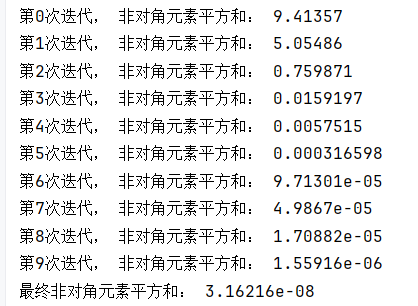
\includegraphics{figs/Jacobi.png}
    \caption{迭代中的非对角元平方和}
\end{figure}\par\noindent
并且可得SDU分解中的各矩阵分别为:
$$ U = 
\left(
    \begin{matrix}
        0.74654& -0.509957& -0.00851348& 0.427257\\
        0.390974& -0.181892& 0.0806777& -0.898635\\
        0.516703& 0.791545& -0.324371& 0.0354674\\ 
        0.151113& 0.283398& 0.942445& 0.0929943\\ 
    \end{matrix}
\right)
$$
$$ \Sigma = 
\left(
    \begin{matrix}
        2.03345 & 0 & 0\\
        0& 0.542556& 0\\
        0& 0& 0.179138\\
        0& 0& 0
    \end{matrix}
\right)
$$
$$ V = 
\left(
    \begin{matrix}
        0.715362& 0.604123& 0.351132\\
        0.426431& -0.775525& 0.465531\\ 
        0.553546& -0.183289& -0.812403\\ 
    \end{matrix}
\right)
$$
经检验, 有$A = U\Sigma V^T$成立.

\subsection{PCA结果}
计算得到的协方差矩阵为:
$$\frac{1}{m}XX^T = 
\left(
    \begin{matrix}
        0.681122& -0.0390067& 1.26519& 0.513458\\
        -0.0390067& 0.186751& -0.319568& -0.117195\\ 
        1.26519& -0.319568& 3.09242& 1.28774\\ 
        0.513458& -0.117195& 1.28774& 0.578532\\
    \end{matrix}
\right)
$$
计算所得的数据存放于压缩包/res目录下, 利用Python matplotlib库进行数据可视化处理, 结果如下:
\begin{figure}[H]
    \centering
    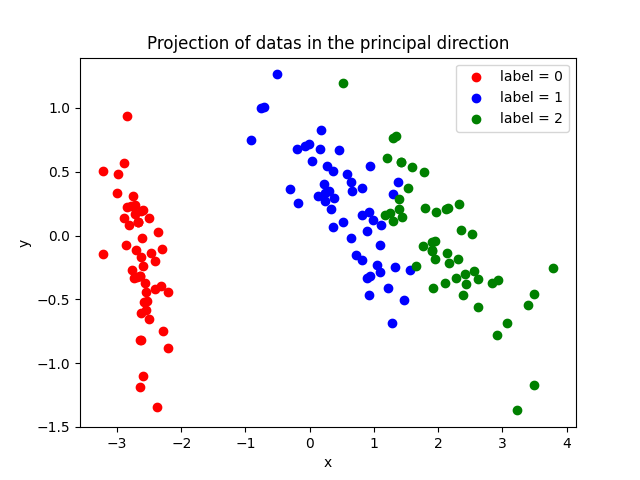
\includegraphics{figs/data.png}
    \caption{数据可视化}
\end{figure}

\section{结果分析}
\paragraph{(a)}  由图1可以看出, 在Jacobi方法执行过程中, 非对角元素平方和呈现逐次下降趋势,
计算$det(AA^T - \lambda_i I)$的结果如下:
\begin{figure}[H]
    \centering
    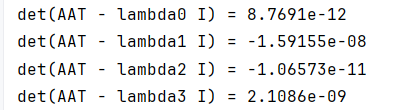
\includegraphics{figs/det.png}
    \caption{计算$det(AA^T - \lambda_i I)$}
\end{figure}
\noindent 上述值均接近0, 可以认为所求的是矩阵$AA^T$的特征值.
\paragraph{(b)} 通过PCA主成分分析后, 可以看出label不同的数据在前两个主方向的投影
区别明显, 说明数据间有显著差异, 其中label = 0的数据与其他两类区别最为明显.

\section{实验总结}
本次实验相比前几次, 任务量有明显提高, 需要自行学习的部分较多. 其中Jacobi方法可以按照教材
所述算法实现(需要注意第三版教材中, Jacobi方法的伪代码有误, 在每次迭代时, a[p][p]与a[q][q]均未置0).
\par 在求出特征值后, 求解特征向量时, 若运用高斯消元法, 可能由于系数矩阵不满秩, 导致解出
平凡解O, 因此在进行列主元消元后, 先判断系数矩阵是否满秩, 若不满秩, 则将后面的全0(接近0)行的解$y_i$先
设置为1.
\par 对于矩阵与其特征值$\lambda_i$, 若$\boldsymbol{v}$是其对应的特征向量, 则$-\boldsymbol{v}$
也是特征向量, 即有两个相反的方向, 因此若直接将特征向量按列拼成矩阵U,V,可能会不符合要求, 
正确的做法是先解出U, 再利用$A=U\Sigma V^T$即$AV = U\Sigma$反解V.

\end{document}